\documentclass[final,5p,twocolumn]{elsarticle}

\usepackage{amssymb}
\usepackage{lineno}

\usepackage{color}
\usepackage{booktabs}
\usepackage{makecell}
\usepackage{pifont}
\usepackage{rotating}
\usepackage{adjustbox}

% \usepackage{graphicx}
% \usepackage{cite}
% \usepackage{url}
% \usepackage{amssymb}

\newcommand{\cmark}{\ding{51}}
\newcommand{\xmark}{\ding{55}}

\newcommand{\todo}[1]{{\color{blue}{#1}}}
\newcommand{\revision}[1]{{\color{black}{#1}}}


\journal{}

\begin{document}
\begin{frontmatter}

\title{AttacKG: Practical CTI Report Parsing \& Threat Intelligence KG Building}


\author[label1]{Zhenyuan Li}
% \author[label2]{Qi Alfred Chen}
% \author[label1]{Runqing Yang}
% \author[label3]{Yan Chen}
% \author[label1]{Wei Ruan}

\address[label1]{Zhejiang University, China}
% \address[label2]{University of California, Irvine, USA}
% \address[label3]{Northwestern University, USA}


\begin{abstract}

\end{abstract}

\begin{keyword}
Cyber Threat \sep Provenance Graph \sep Intrusion Detection \sep Digital Forensic
\end{keyword}

\end{frontmatter}

% \linenumbers

%% main text
\section{Introduction}
\label{sec:introduction}

\subsection{Background}

\ToDo{1 Cyber attacks are diversifying.}

\ToDo{2 Threat intelligence and threat reports are helpful tools}

Provenance graph as a threat representation tool are already widely studied and adopted \cite{li2021}. With provenance graph, security analyzers are able to encode system execution history into graphs. Thus provenance graph contain rich semantic information. However, there are still a gap between provenance graphs and human understandable information. Poirot \cite{Milajerdi2019} try to solve this problem by involve TTPs and kill chain proposed by MITRE \cite{}.

\ToDo{3 Provenance graph are widely-used and recongnized threat representation approach.}

\subsection{Related Works}

\ToDo{1 Compare with existing automated threat intelligence collection works.}

\ToDo{2 How our work support provenance graph-based threat detection.}

\subsection{Our work}

\ToDo{1 Extracting incomplete attack graph from single CTI report.}

\ToDo{2 Delineating behavioural and clustering analysis.}

\ToDo{3 Implement applicaitons.}

\subsection{Contribution}

\ToDo{1 New threat intelligence representation approach.}

\ToDo{2 Automated threat intelligence collection and management system.}

\ToDo{3 Collected a large amount of threat intelligence and done a through analysis by real-word application.}

\ToDo{4 We provided a open attack dataset.}


\begin{figure}
    \centering
    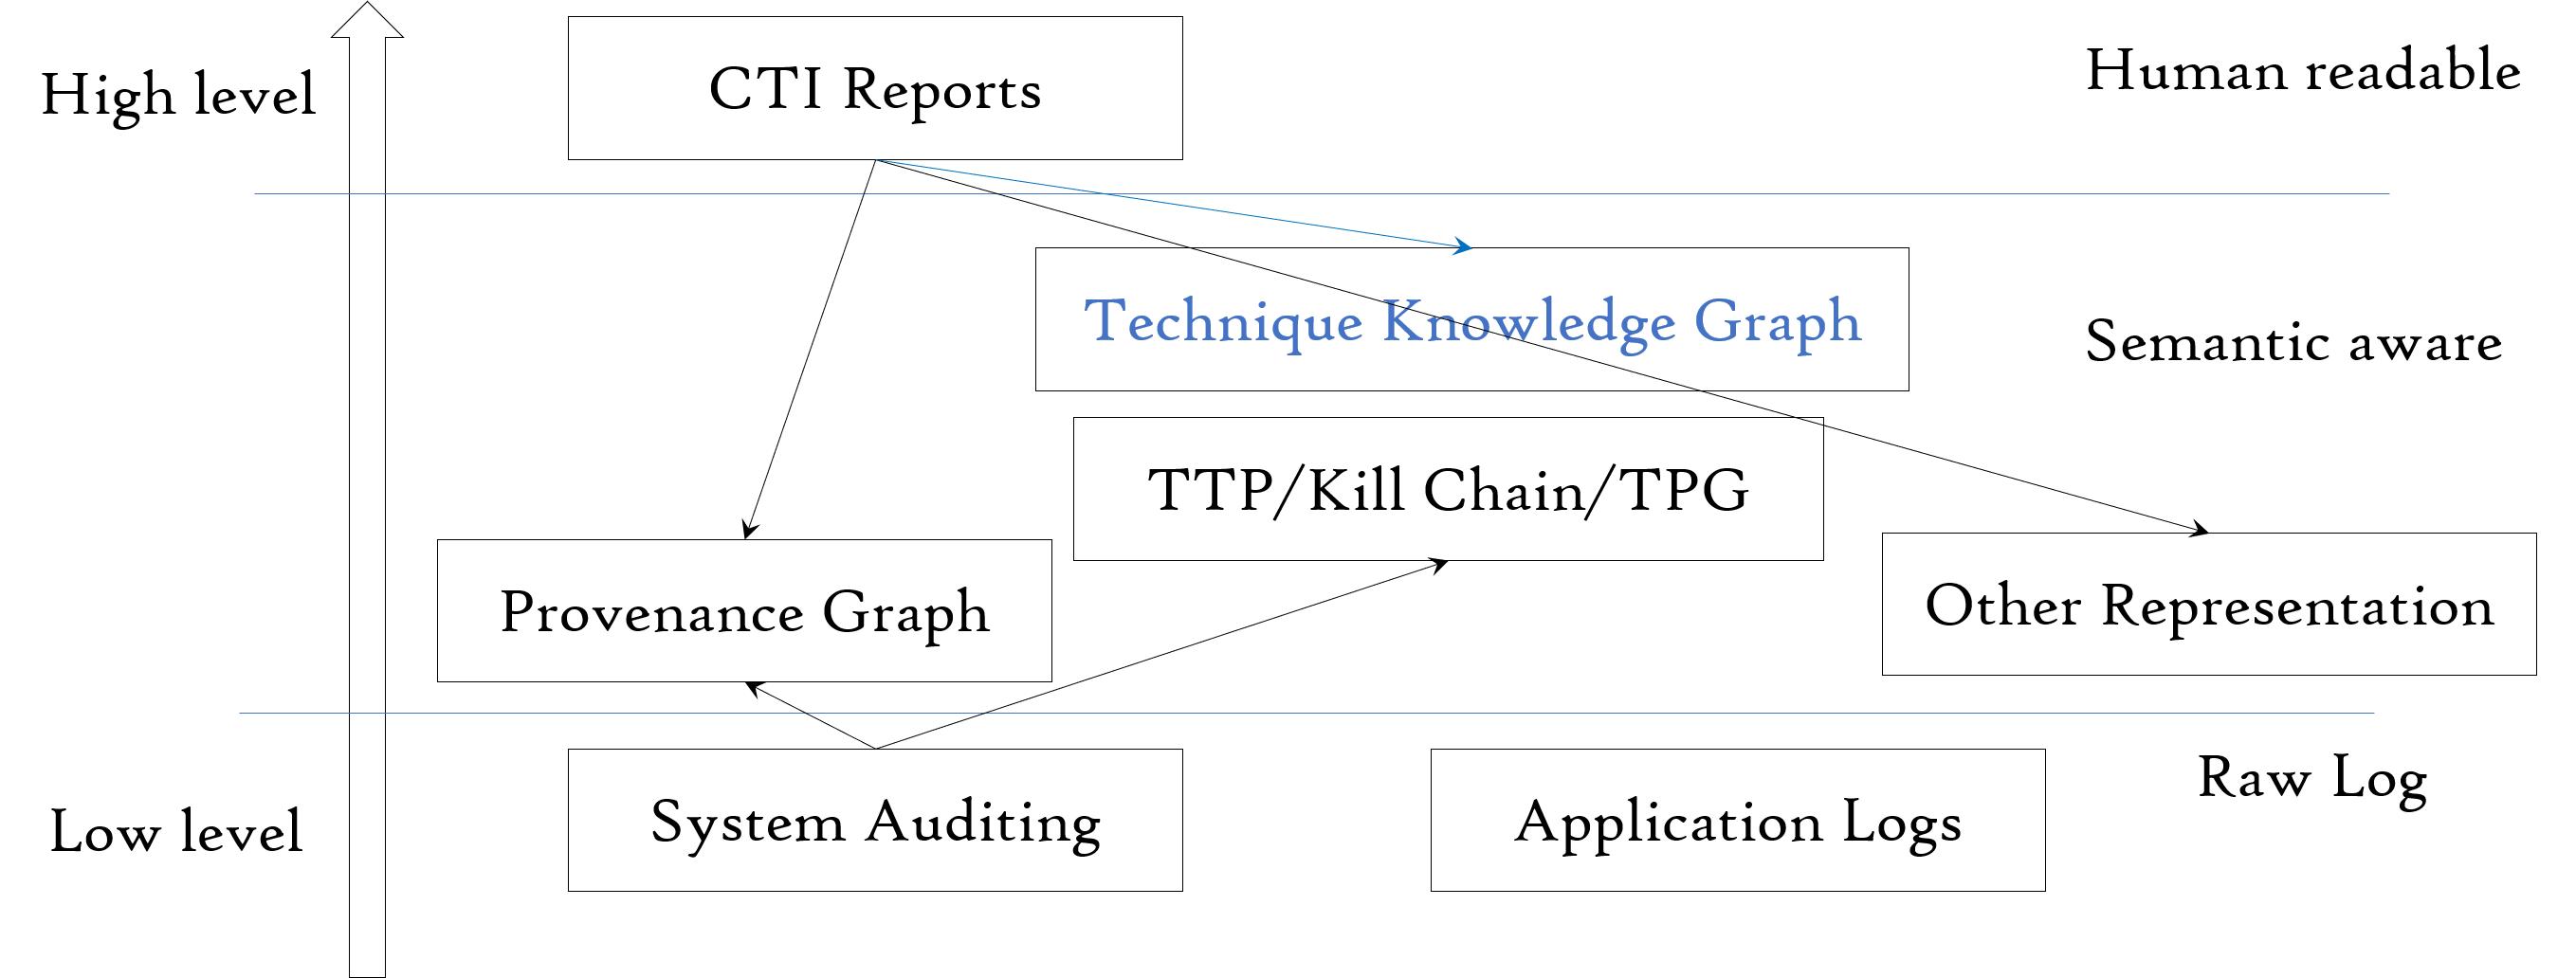
\includegraphics[width=3.5in]{Image/representation.png}
    \caption{Different Representation of Cyber Attacks.}
    \label{fig:representation}
\end{figure}

\section{Background}
\label{sec:background}

\subsection{Three granularity of variant for PG}

\ToDo{1 Different combination of attack techniques.}

\ToDo{2 Different mplementation of attack techniques.}

\ToDo{3 Different option for attack nodes.}
\cite{Michael2021} \cite{Kurogome2019}

\subsection{Problem statement}

CTI reports contain rich information needed by detection and analyzer. However, existing reports analysis work focus only on the reports itself, leave out lots of useful information. We propose to adopt TTPs knowledge and Technique/Tactic Knowledge Graph(TKG) to organize the knowledge extracted from reports. And generate more useful attack descriptions.

On the one hand, current CTI sources focus on naïve IoCs, such as bad IPs, malware hashes, etc., without much high-level semantic. Such CTI are neither general nor reliable. \cite{Li2019} On the other hand, unstructed threat whitepapers are vague. – We need new CTI standards. 

On the other hand, effective(fast) and efficient(accuracy) detection require accurate attack description. State-of-the-art work rely on manual analysis \cite{Milajerdi2019} which is difficult to expand. – We need more and automated CTI. 

\subsection{Challenges}

\ToDo{C1. How to extract Techniques from Natural-Language CTI? – \S\ref{sub_sec:nlp_parser}}
% Contribution 1: Automated report parsing. S: TTPs templates (knowledge base) vs. Patterns in CTI (NLP)

C1-1. Unstructured Threat Whitepapers Are Vague: 

Vague nodes: Lack of explicit node identification; Vague subject: 

Vague edges: An operation may corresponds to a series of edges in PG

C1-2. How to find technique dependencies? (Sometimes)
S: Employ System Entity/Report/self-defined tags(TCP sockets) as connections

\ToDo{C2. How to integrate multiple CTI reports? – Contribution 2: Building attack Technique Knowledge Graph. -\S\ref{sub_sec:TKG_update}}

Observations:

1. A single report most likely covers a fragment of an APT attack?

2.Different reports may conflict due to variant malwares


\ToDo{C3. How to use the TKG?  - What basic function we need to implement on TKG? -\S\ref{sec:case_study}}

\section{Related Work}
\label{sec:relatedworks}

\subsection{Threat Intelligence}

Threat intelligence are widely adopt in both academia and industry. \cite{Berady2021,Michael2021} 

\subsection{Extract threat intelligence from unstructured CTI reports}

Existing works try to extract IoC \cite{Liao}, TTPs \cite{Husari2017}, Attack Chains \cite{Zhu2018}, Attack Graph \cite{Gao} from unstructed TI. Most recent works tend to extract more detailed and structure information. Ideal CTI should be general to cover more attack cases while detailed to avoid FP. To strike a balance, we need to correlate related attack descriptions and construct a better one.

However, single CTI report cannot provide 

\subsection{Modeling the cyber threat intelligence (Knowledge graphs for security purpose)}

\cite{Gao2020,Zhao2020} try to model and quantify the underlying relationship among heterogeneous IoCs (Attackers, Device, Platform, Vulnerability, File, Type). These works do not include information about how these IoCs work together (PG), and leave lots of details.

\subsection{Threat detection and forensic (Adopt graphs to represent cyber attacks)}

\cite{Milajerdi2019}, etc. can adopt threat intelligence extracted by our system. Accurate and general attack description can ensure detection efficiency and accuracy.
\section{Technique Knowledge Graph}
\label{sec:tkg}

\subsection{TKG design}

The TKG should take a hierarchical (two-layer) design, namely, system entity (and action) level and TTP level. On system entity level, the TKG looks just like many sub-graphs(TPG) of Provenance Graph.  Every sub-graph represents a TTP and make up the TTP-level TKG. Every TTP node should have one or more inputs and outputs. And we can use these inputs and outputs connect TTPs.


\subsubsection{Layer 1: kill chain layer}

\subsubsection{Layer 2: TTP representation layer}

\subsection{Initing the TKG – The Workflow:
}

\begin{figure}
    \centering
    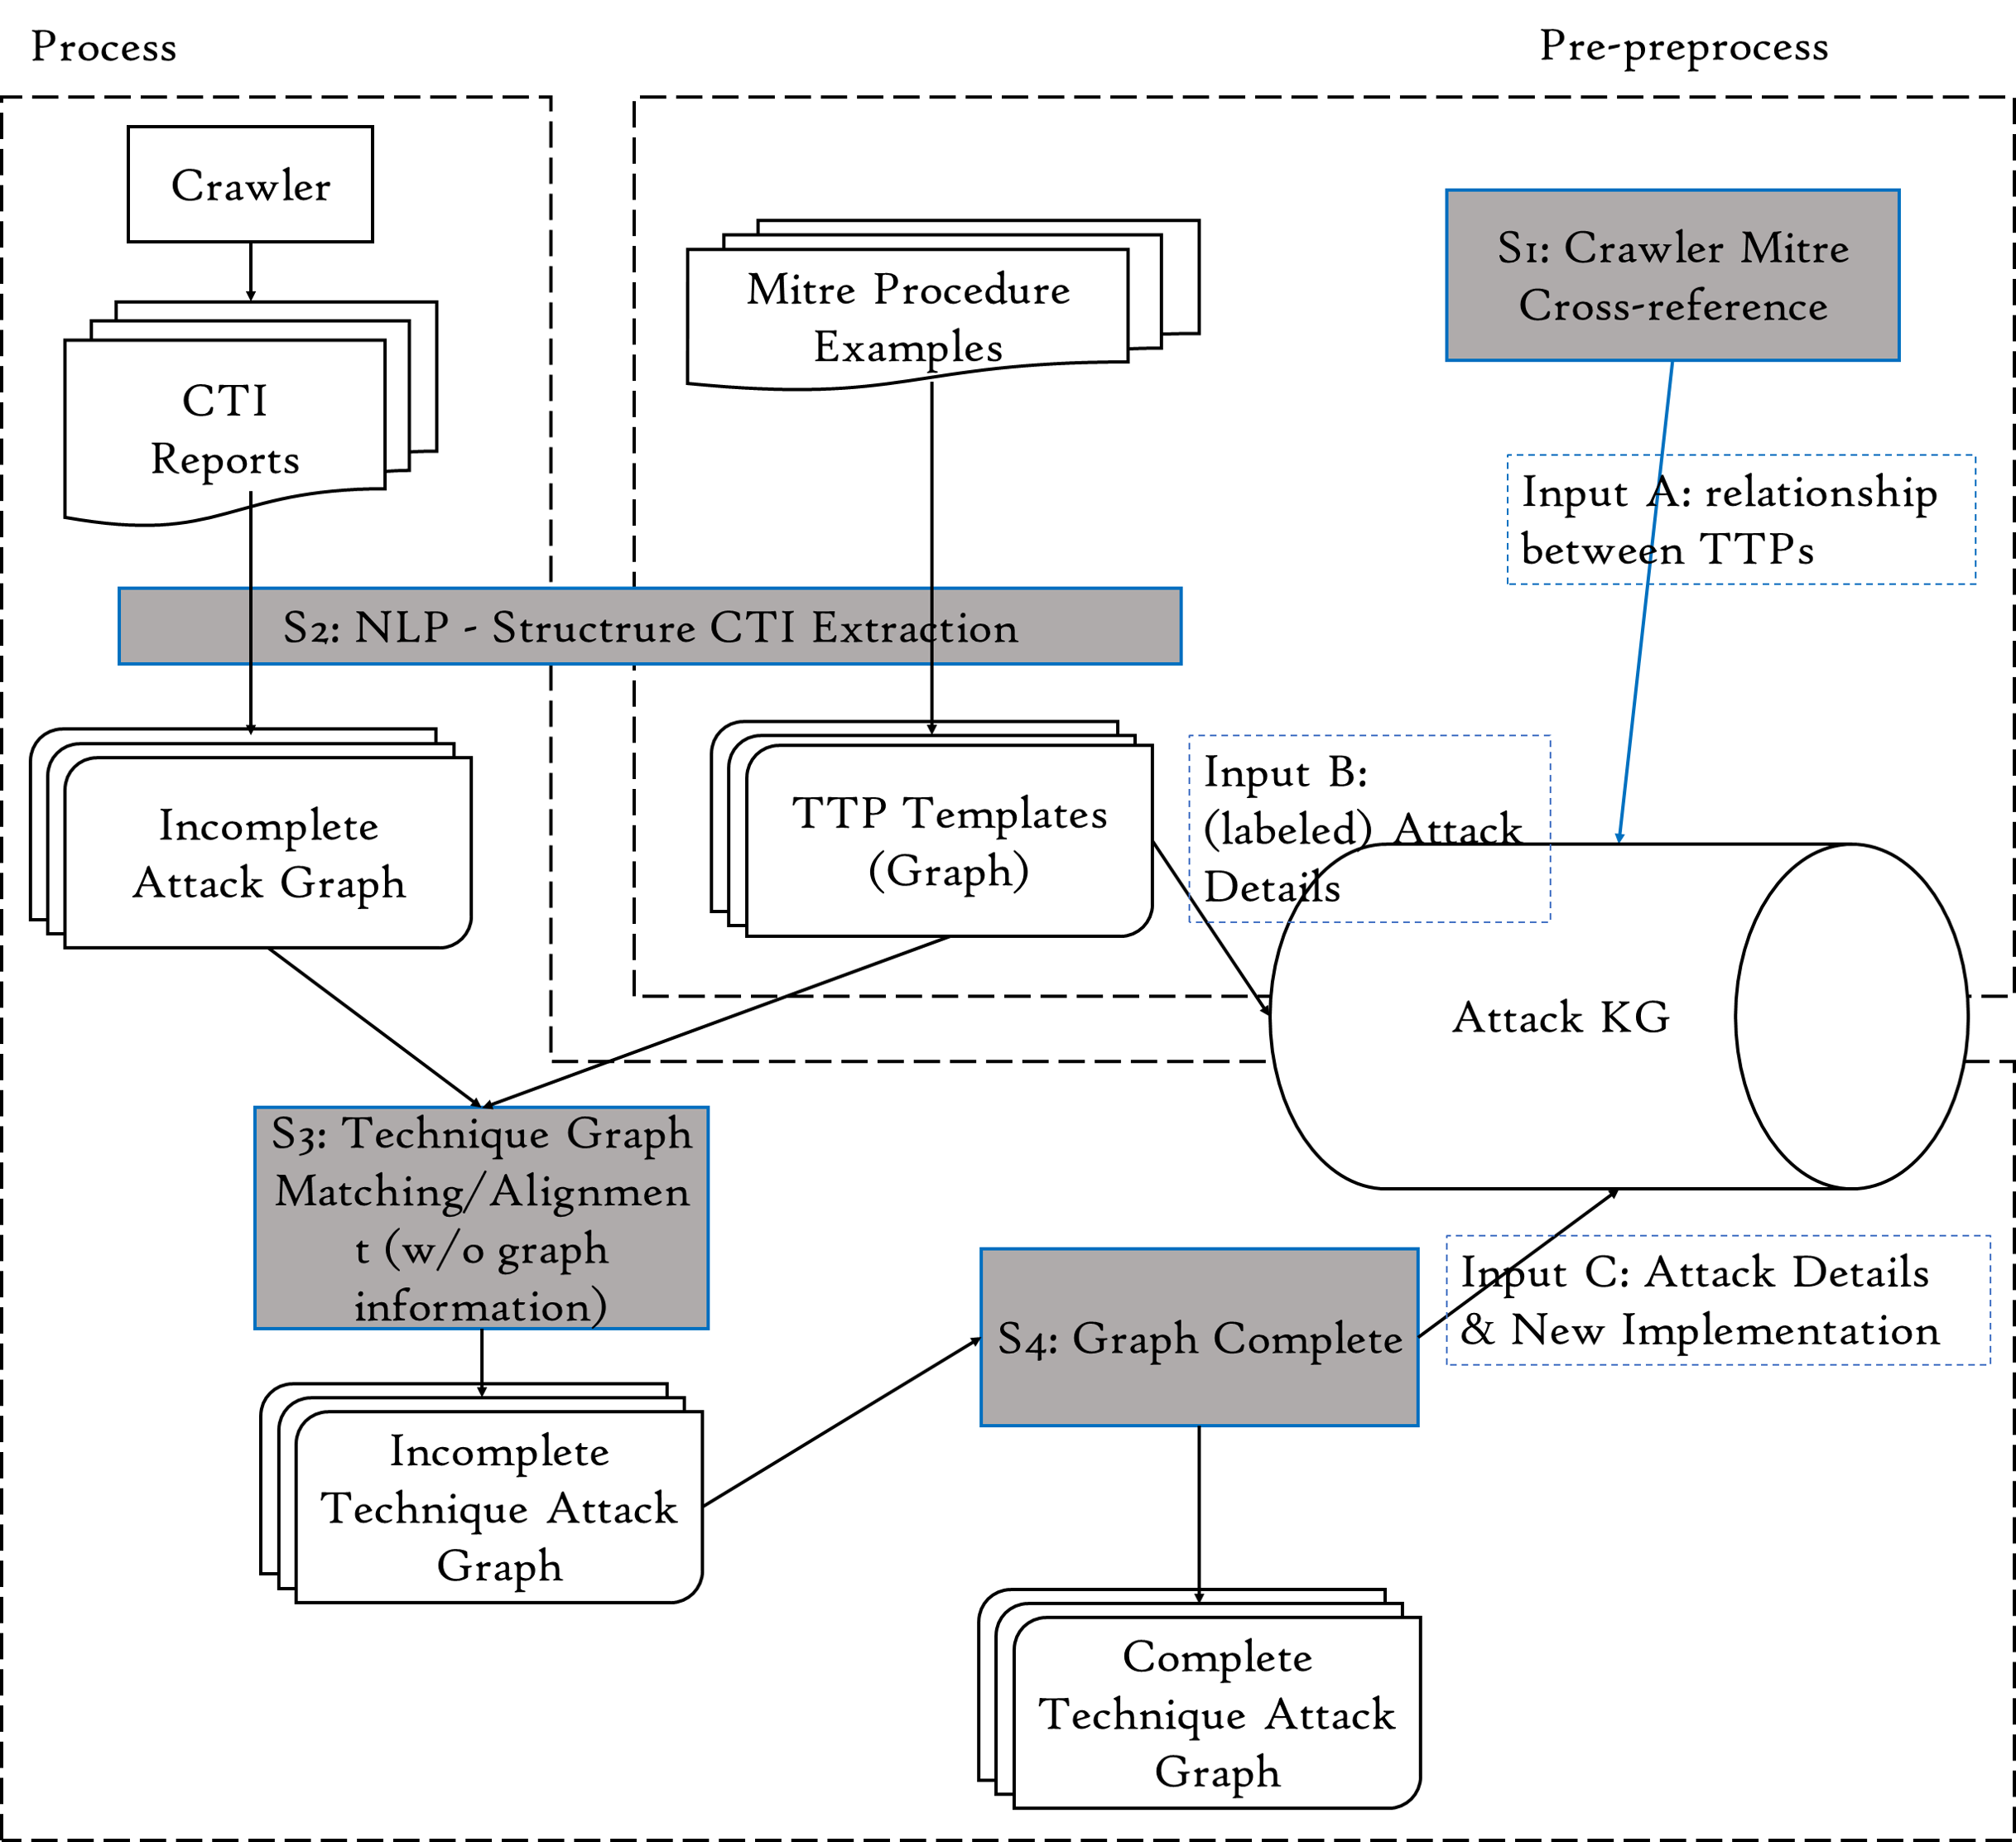
\includegraphics[width=3.3in]{Image/architecture.png}
    \caption{Attack Knowledge Graph Building Process.}
    \label{fig:architecture}
\end{figure}

\subsubsection{NLP-based CTI report parsing: the input is CTI reports and description for all the TTPs (mitre attack)}
\label{sub_sec:nlp_parser}

\begin{figure}
    \centering
    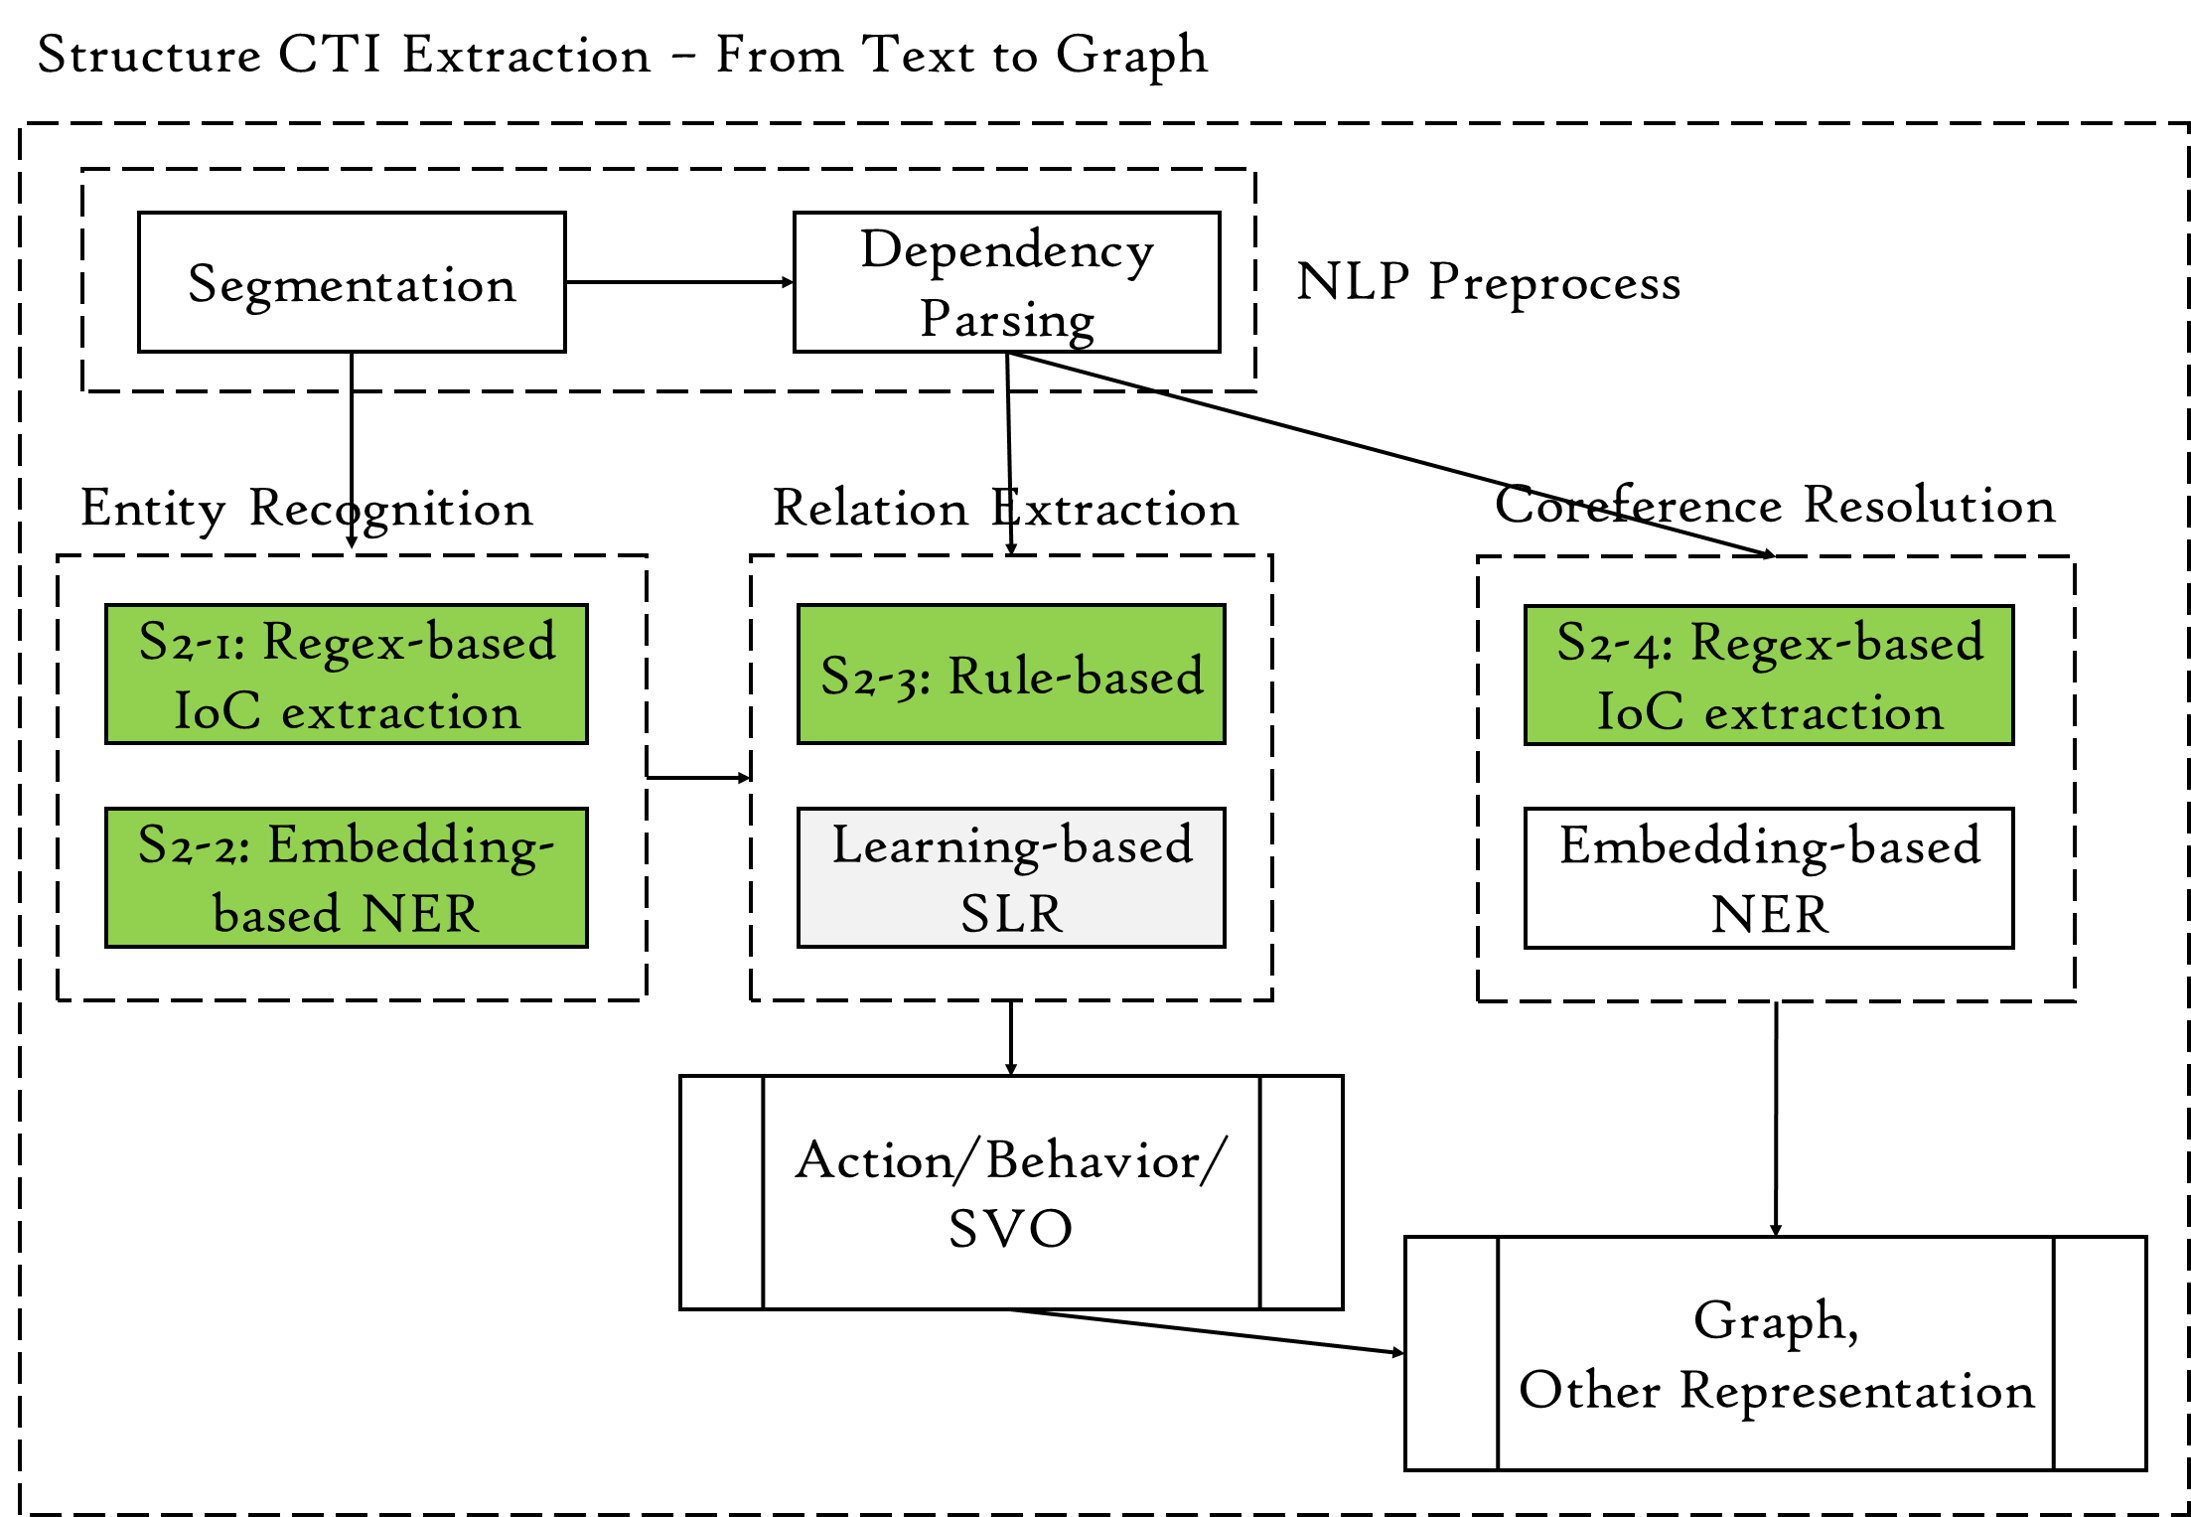
\includegraphics[width=3.3in]{Image/nlp_architecture.png}
    \caption{NLP-based Report Parsiing Process.}
    \label{fig:nlp_architecture}
\end{figure}

\ToDo{S2-0. Preprocess}

\ToDo{S2-1,2. NLP-based TTP extraction}

\ToDo{S2-3. Relation extraction}

\ToDo{S2-4. Co-reference resolution}

\ToDo{S2-5. Attack graph reconstruction for each TTP segment}

\subsubsection{TKG initialization-update-loop: the input is subgraphs representing TTPs}
\label{sub_sec:TKG_update}


\ToDo{1 Find similar subgraphs in TKG according to TTP, input/output, IoCs, subgraph structure.}

\ToDo{2 If not match, add subgraphs to the TKG; If match, find the difference and try to abstract a more general model to match both graph.}

\ToDo{3 Try to connect the new TTP with other TTPs according to the inputs and outputs.}

\subsection{TKG matching}
\label{sub_sec:matching}

\ToDo{Speed up the matching process by key nodes matching.}

\section{TKG Case Study}
\label{sec:case_study}

\subsection{TKG can help with the detection of threat}

\subsection{TKG can help with the understanding of threat}

\section{Discussion}
\label{sec:discussion}


\section{Conclusion}
\label{sec:conclusion}


\section*{Acknowledgment}
We would like to thank the anonymous reviewers for providing valuable feedback on our work. This work is supported by the Zhejiang Lab’s International Talent Fund for Young Professionals.

%% The Appendices part is started with the command \appendix;
%% appendix sections are then done as normal sections
%% \appendix


\bibliographystyle{elsarticle-num-names} 
\bibliography{Attack}


\end{document}
\endinput

